%----------------------------------------------------------------------------------------
%	PACKAGES AND DOCUMENT CONFIGURATIONS
%----------------------------------------------------------------------------------------

\documentclass[11pt]{article}

\usepackage[english]{babel}
\usepackage[utf8]{inputenc}
\usepackage[T1]{fontenc}
\usepackage[top=3cm, bottom=3cm, left=2.5cm, right=3.5cm]{geometry}
\usepackage{graphicx}
\usepackage[babel=true]{csquotes} % csquotes va utiliser la langue définie dans babel

\setlength\parindent{0pt} % Removes all indentation from paragraphs

\begin{document}

\begin{center}
\begin{large}
\textsl{LifeBand : Presentation} \\
\end{large}
.............................................................. \\
\end{center}

\paragraph{} This guide presents what LifeBand is and what it can do.

\begin{tabular}{p{6.5cm}p{10cm}}
\begin{center}
Fig. 1 \newline
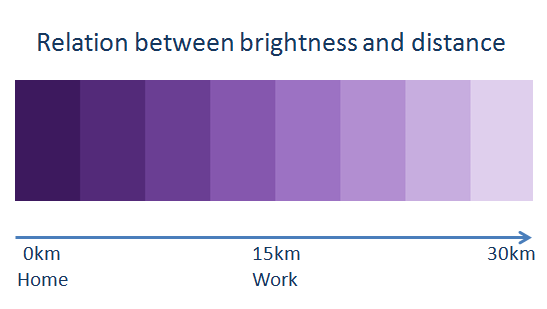
\includegraphics[width=6cm]{scale.png}\newline\newline
Fig. 2 \newline
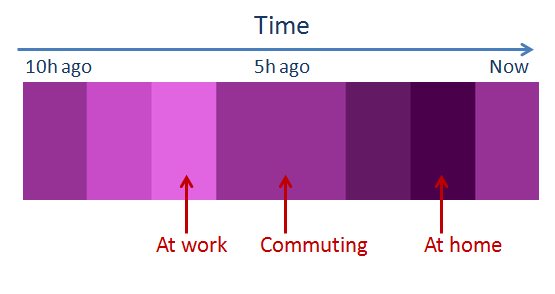
\includegraphics[width=6cm]{timeline.png}\newline\newline
Fig. 3 \newline
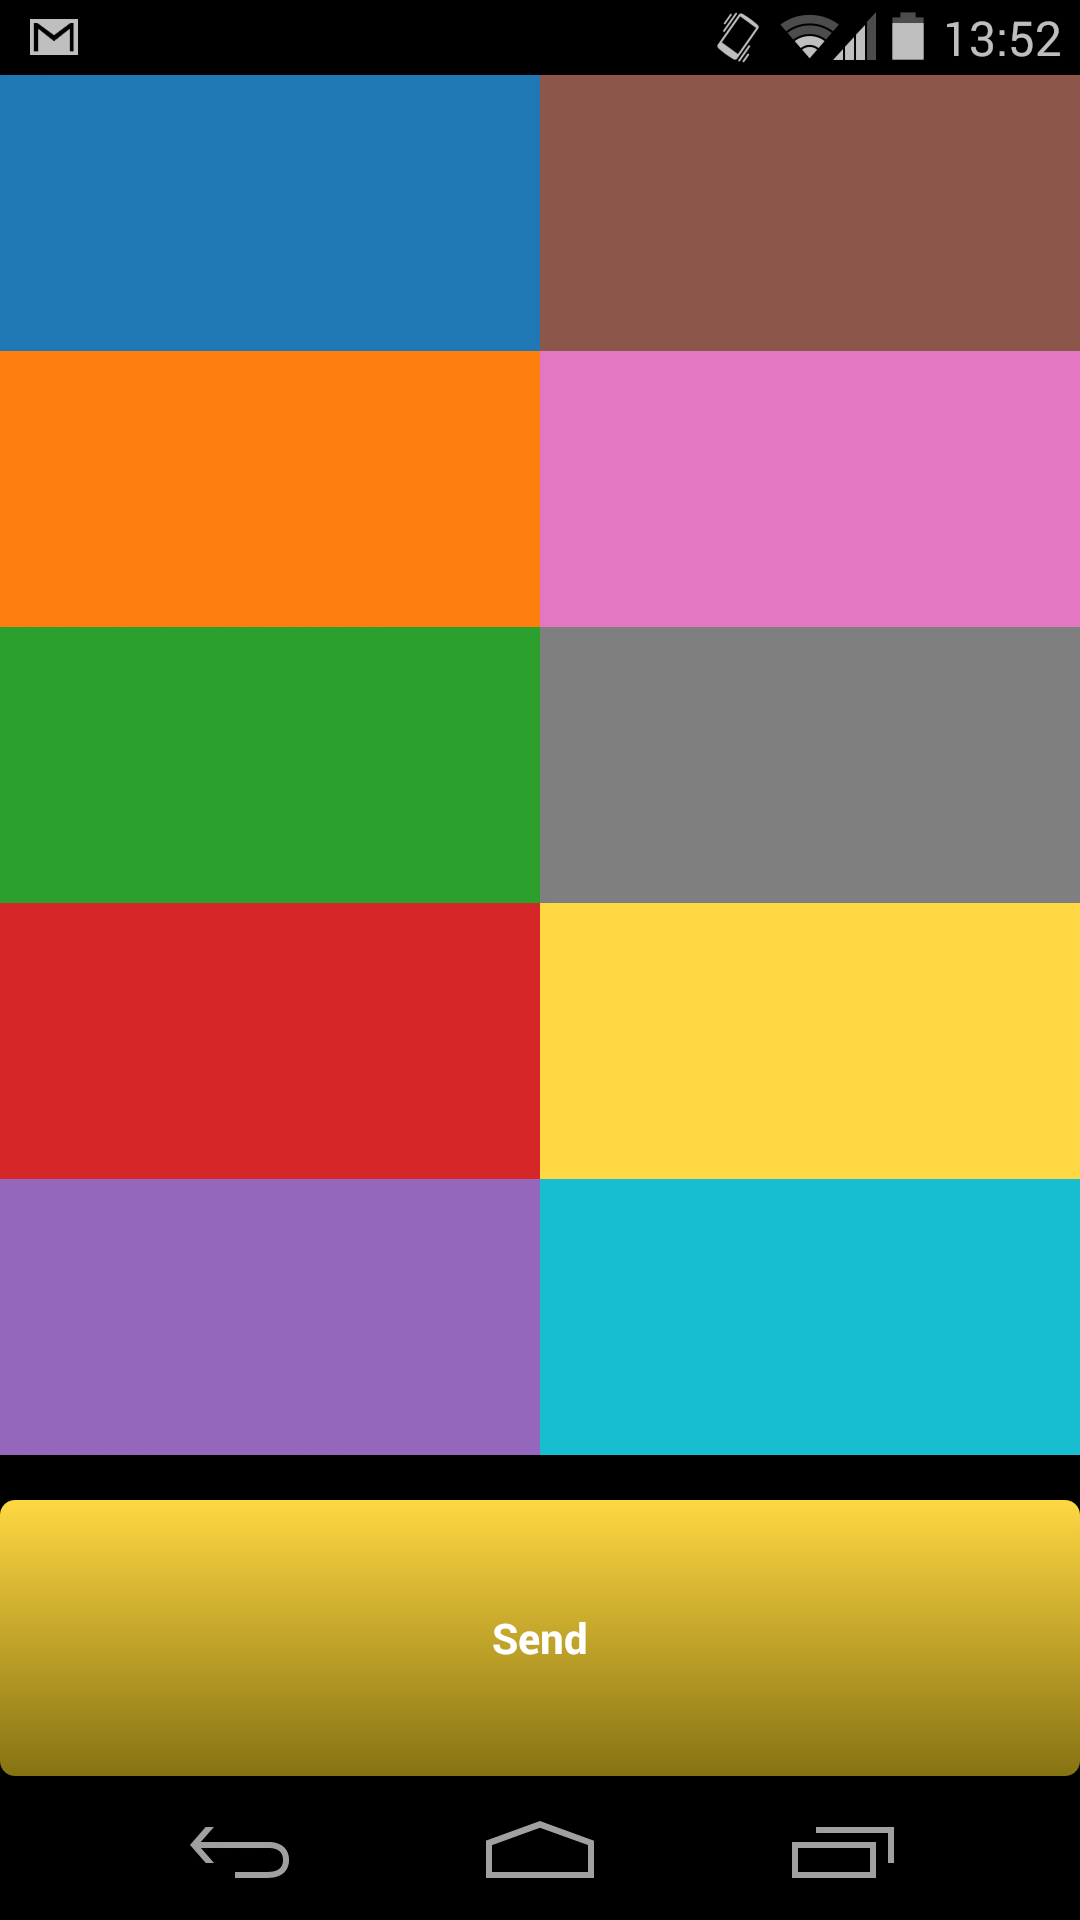
\includegraphics[width=3cm]{color.png}\newline\newline
Fig. 4 \newline
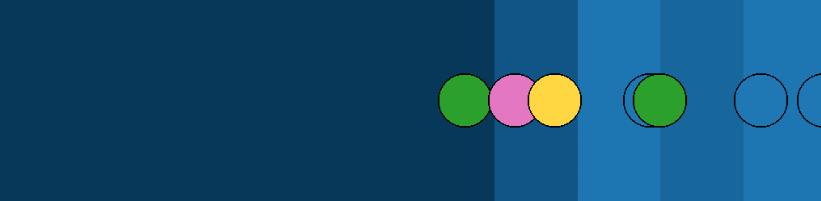
\includegraphics[width=5.8cm]{nudges.png}\newline
\end{center}
&
\paragraph{Passively sharing location information}
\paragraph{} The LifeBand is an application that shows up as a band with colors that represent location information from your partner. With it you will be able to know when your partner is available, when he is sleeping or commuting for example. The application runs in background on your smartphone and passively share location information. It requires 3G or Wifi but uses a small amount of data.
\paragraph{} To maintain your privacy, the shared information is not your precise location, but just an indication of your distance to home. The brightness is used to show how close or far away you are. Dark means a small distance from home while light means a long distance from home. Fig. 1 shows the scale for someone who works at 15km from his home.
\paragraph{} The band is also a timeline of the information explained on Fig. 2. The present instant is displayed at the far right; The full band displays 10 hours of data.

\paragraph{Sending color nudges}
\paragraph{} The application has an active part that allows you to send nudges containing colors. This is done by selecting a color on the screen Fig. 3 and pressing SEND. The nudge appears as a dot on the band as shown in Fig. 4.

\end{tabular}
\vfill
\begin{center}
.............................................................. \\
Université Paris Sud - LRI - in|situ|
\end{center}

\end{document}